%! suppress = LineBreak
%! suppress = MissingLabel
\section{Методы эволюции нейронных сетей}\label{sec:evolutionMethods}

Существует множество алгоритмов для эволюции нейронных сетей. Они классифицируются по схемам кодирования и тому, модифицируют ли они веса, топологию или и то, и другое. Однако не все они пользуются популярностью и имеют хорошие библиотеки с реализацией. Можно выделить два алгоритма NEAT\cite{s1} и HyperNEAT\cite{s16}, которые находят своё применение до сих пор и имеют регулярно обновляемые библиотеки.

\subsection{NEAT}

Название этого алгоритма расшифровывается как нейроэволюция расширяющихся топологий (NeuroEvolution of Augmenting Topologies). Это метод, предназначенный для эволюции искусственных нейронных сетей с помощью генетического алгоритма. Главная идея NEAT заключается в том, что эволюцию наиболее эффективно начинать с маленьких и простых сетей, которые постепенно становятся всё более сложными с каждым поколением.

Алгоритм основан на трех ключевых принципах. Во-первых, для того чтобы позволить структурам нейронных сетей усложняться с течением поколений, необходим метод отслеживания того, какой ген является каким. В противном случае в последующих поколениях будет неясно, какая особь с какой совместима и как их гены должны быть объединены для получения потомства. NEAT решает эту проблему, присваивая уникальную историческую метку каждому новому элементу структуры сети, который появляется в результате структурной мутации. Историческая метка – это число, присвоенное каждому гену в соответствии с порядком его появления в ходе эволюции. Эти числа наследуются без изменений во время скрещиваний и позволяют NEAT выполнять скрещивание без необходимости трудоемкого топологического анализа. Таким образом геномы различной организации и размеров остаются совместимыми на протяжении всей эволюции, что решает ранее открытую проблему сопоставления различных топологий в эволюционирующей популяции. 

Во-вторых, NEAT разделяет популяцию на виды таким образом, что отдельные особи конкурируют в основном внутри своих собственных ниш, а не с популяцией в целом. Благодаря этому топологические инновации защищены и имеют время оптимизировать свою структуру, прежде чем конкурировать с другими нишами в популяции. NEAT использует исторические метки на генах, чтобы определить, к какому виду принадлежат различные особи. 

В-третьих, в отличие от других существующих систем эволюции нейронный сетей алгоритм NEAT начинается с однородной популяции простых сетей без скрытых узлов. Возникает новая топологическая структура по мере того, как происходят структурные мутации, и выживают только те структуры, которые признаны полезными в результате оценки функцией приспособленности. Таким образом NEAT выполняет поиск топологических структур, начиная с самых простых, и находит оптимальную структуру для решения задачи.\\
%
Плюсы алгоритма:
\begin{enumerate}[--]
    \item Наличие актуальных библиотек с реализацией на разных языках программирования: C\#, C++, Python и другие.
    \item Операции мутации и скрещивания применяются не только к весам, но и к топологии нейронной сети.
    \item Подходит для трудно формализируемых задач, где функция потерь и функция приспособленности могут быть не определены.
\end{enumerate}
%
Минусы алгоритма:
\begin{enumerate}[--]
    \item Медленно сводится к оптимальному решению, если условия задачи очень сложны. 
    \item Плохо масштабируется из-за прямой схемы кодирования. Эффективно работает только с нейронными сетями малого размера, у которых меньше 200 узлов. 
\end{enumerate}

\subsection{HyperNEAT}

Полное название этого алгоритма можно перевести как нейроэволюция расширяющихся топологий, основанная на гиперкубе (Hypercube-based NeuroEvolution of Augmenting Topologies). HyperNEAT является дополнением NEAT и использует непрямую схему кодирования нейронных сетей для решения проблемы плохой масштабируемости.

Для непрямого кодирования используются субстрат и сети, производящие составные паттерны:

\begin{enumerate}[label=\textbullet]
    \item Субстрат -- это некоторое геометрическое упорядочивание узлов нейронной сети. Самый простой вариант такого упорядочивания -- решетка, где каждая отдельная точка $(x,y)$ является узлом (Рисунок~\ref{SubstratConfig}). 
    
    \begin{figure}[ht]
        \begin{center}
            \scalebox{0.4}{
                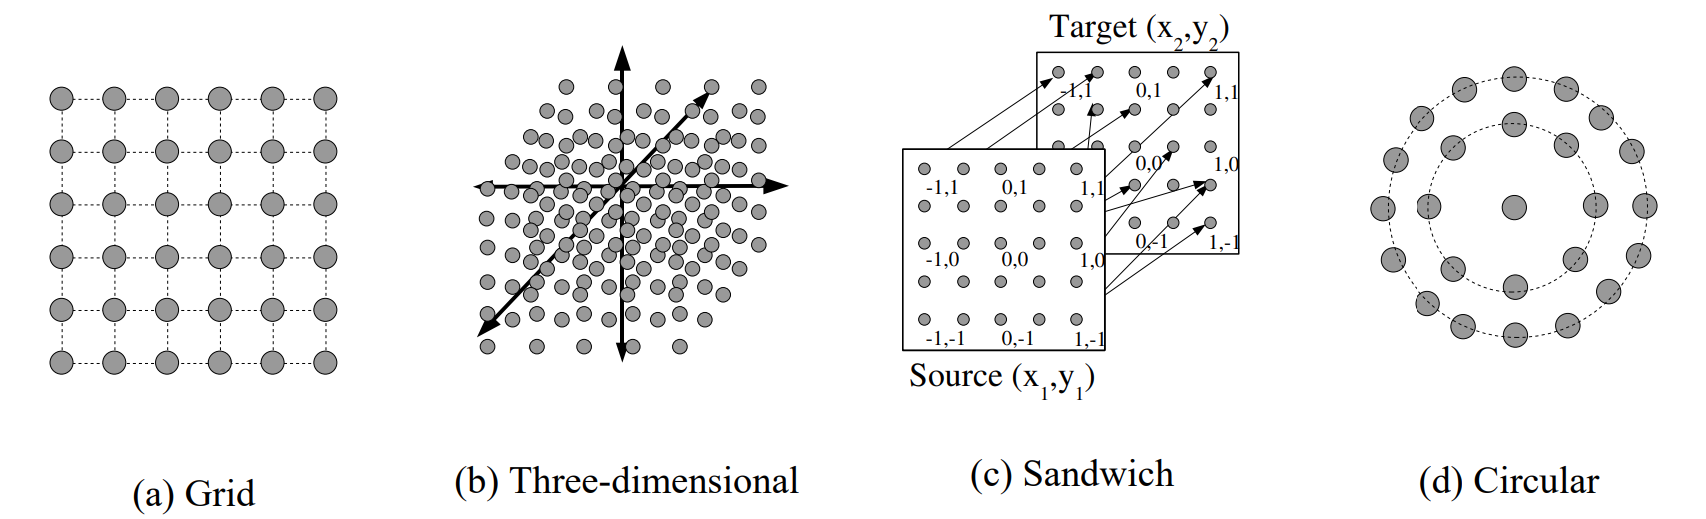
\includegraphics{images/SubstratConfig}
            }
    
            \caption{
                \label{SubstratConfig}
                Варианты субстратов.}
        \end {center}
    \end {figure}
    
    \item Сети, производящие составные паттерны (Compositional pattern-producing networks, далее – CPPN) -- это разновидность искусственных нейронных сетей. Основная особенность CPPN в том, что в их узлах могут использоваться разные функции активации. Выбор конкретного множества функций активации зависит от желаемых паттернов и закономерностей (Рисунок~\ref{CPPNvsANN}).
    \begin{figure}[ht]
        \begin{center}
            \scalebox{0.28}{
                \includegraphics{images/СPPNvsANN}
            }

            \caption{
                \label{CPPNvsANN}
                Разница между обычной нейронной сетью и CPPN.}
        \end {center}
    \end {figure}
\end{enumerate}



Алгоритм получения нейронной сети из субстрата описывается следующим образом (Рисунок~\ref{substrat}):

\begin{enumerate}
    \item Получи координаты $(x,y)$ каждой возможной пары узлов в субстрате.
    \item Подай эти пары координат на вход в CPPN, которая была получена в результате работы алгоритма NEAT.
    \item CPPN выдаст вес между каждой возможной парой узлов. Если вес между некоторой парой узлов выше определенного значения, то ребро между ними существует, если нет, то ребро игнорируется.
\end{enumerate}

\begin{figure}[ht]
    \begin{center}
        \scalebox{0.5}{
            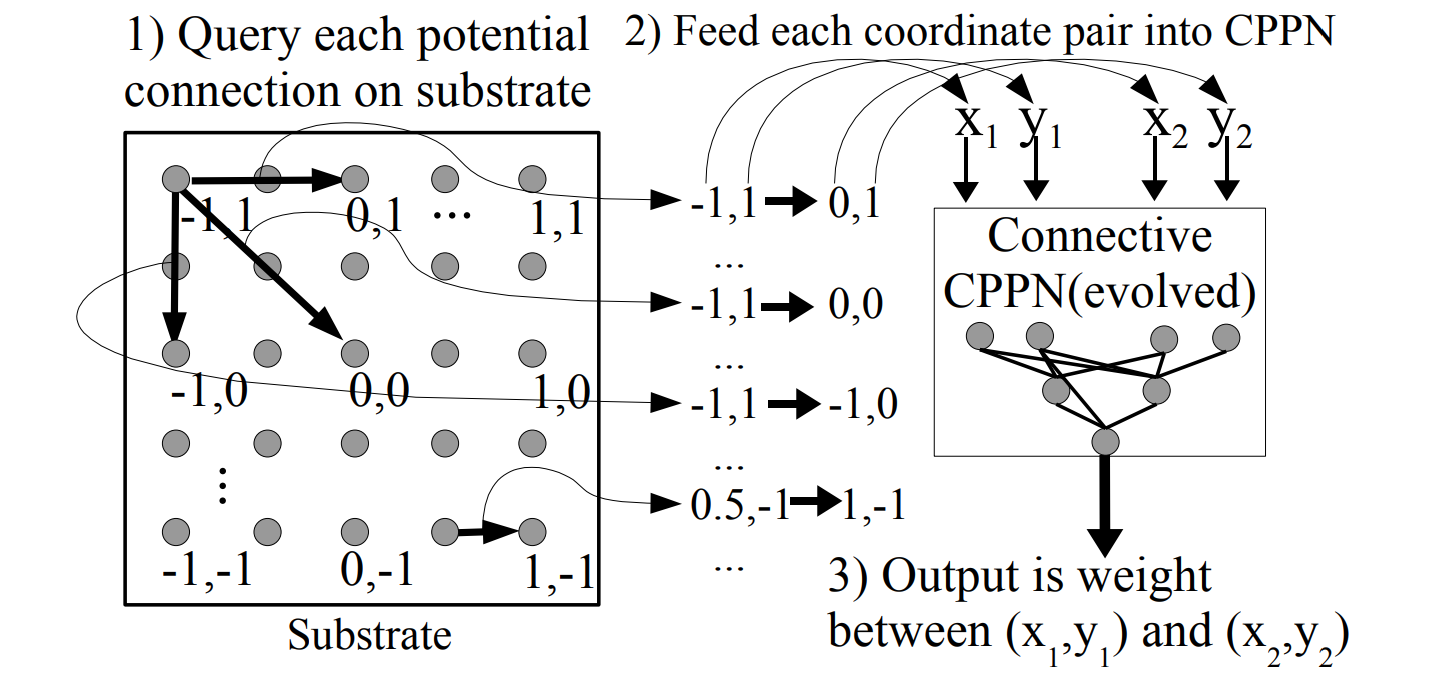
\includegraphics{images/substrat}
        }

        \caption{
            \label{substrat}
            Алгоритм получения нейронной сети из субстрата с помощью CPPN.}
    \end {center}
\end {figure}


{\parindent0pt Плюсы метода HyperNEAT:}
\begin{enumerate}[--]
    \item Наличие актуальных библиотек с реализацией на разных языках программирования: C\#, C++, Python и другие.
    \item Подходит для трудно формализируемых задач, где функция потерь и функция приспособленности могут быть не определены.
    \item Способен работать с очень большими нейронными сетями.
\end{enumerate}
%
Минусы метода HyperNEAT:
\begin{enumerate}[--]
    \item Для работы алгоритма пользователю требуется выбрать субстрат, определяющий множество возможных топологий нейронных сетей. 
    \item Намного медленнее, чем NEAT, поскольку требуется больше шагов для создания нейронных сетей на каждом из поколений.
\end{enumerate}


\subsection{Вывод}
Проанализировав плюсы и минусы обоих алгоритмов, было решено использовать NEAT, так как:

\begin{enumerate}[label=\textbullet]
    \item Нет необходимости в работе с большими нейронными сетями, поскольку оружие представляется простыми сетями, у которых только 3 ввода и 5 выводов.
    \item NEAT не использует субстрат, что позволяет генерировать сети произвольной топологии.
\end{enumerate}








